% =====================================================================
\chapter{Primitivas e integral de Riemann}
\label{tema:1}
% =====================================================================

El cálculo integral responde a dos preguntas que, en apariencia, no tienen relación: qué función tiene una derivada dada y cuánto vale el área bajo una curva. Este tema plantea las dos por separado. La primera conduce a las primitivas; la segunda, a la integral de Riemann, definida como el número que queda atrapado entre las sumas inferiores y superiores de rectángulos. El teorema fundamental del \cref{tema:2} mostrará que ambas preguntas son la misma. La exposición sigue los capítulos~13 de Spivak~\cite{spivak} y~1 de Apostol~\cite{apostol}, con los ejemplos y ejercicios de las §5.1 y~5.2 de~\cite{openstax1}, de la §5.5 de Strang~\cite{strang} y de la parte~A de la unidad~3 del curso 18.01SC del MIT~\cite{mit1801}.

\section{Primitivas}

\begin{definicion}[Primitiva]\label{def:primitiva}
Sea $I\subseteq\R$ un intervalo y sea $f\colon I\to\R$. Una función $F\colon I\to\R$ es una \emph{primitiva} de $f$ en $I$ si $F$ es derivable en $I$ y $F'(x)=f(x)$ para todo $x\in I$. El conjunto de todas las primitivas de $f$ se denota $\int f(x)\dif x$ y se llama \emph{integral indefinida} de $f$.
\end{definicion}

\begin{proposicion}\label{prop:primitivas-constante}
Sean $F$ y $G$ dos primitivas de $f$ en un intervalo $I$. Existe una constante $C\in\R$ tal que $G(x)=F(x)+C$ para todo $x\in I$. En consecuencia, si $F$ es una primitiva, $\int f(x)\dif x=\{F+C: C\in\R\}$, lo que se escribe abreviadamente $\int f(x)\dif x=F(x)+C$.
\end{proposicion}

\begin{proof}
La función $H=G-F$ es derivable en $I$ con $H'=f-f=0$. Sean $x<y$ dos puntos de $I$. Como $I$ es un intervalo, $[x,y]\subseteq I$, y el teorema del valor medio de Lagrange (módulo~0.5) da un $c\in(x,y)$ con $H(y)-H(x)=H'(c)(y-x)=0$. Luego $H$ toma el mismo valor $C$ en todos los puntos de $I$.
\end{proof}

La hipótesis de que $I$ sea un intervalo es imprescindible. En $\R\setminus\{0\}$, la función $H(x)=0$ si $x<0$ y $H(x)=1$ si $x>0$ tiene derivada nula y no es constante; por eso las primitivas de $1/x$ en $\R\setminus\{0\}$ son $\ln\abs{x}+C_1$ para $x<0$ y $\ln\abs{x}+C_2$ para $x>0$, con constantes independientes.

Como la derivada es lineal, también lo es la integral indefinida: si $F$ y $G$ son primitivas de $f$ y $g$, entonces $\alpha F+\beta G$ es primitiva de $\alpha f+\beta g$. Leyendo al revés la tabla de derivadas del módulo~0.5 se obtienen las \emph{primitivas inmediatas} de la \cref{tab:inmediatas}; cada fila se comprueba derivando la columna derecha.

\begin{table}[h]
\centering
\small
\begin{tabular}{@{}lll@{}}
\toprule
$f(x)$ & $\int f(x)\dif x$ & Validez \\
\midrule
$x^{r}$, $r\neq-1$ & $\dfrac{x^{r+1}}{r+1}+C$ & $x>0$ (todo $x$ si $r\in\N_0$) \\[4pt]
$\dfrac1x$ & $\ln\abs{x}+C$ & cada intervalo de $\R\setminus\{0\}$ \\[4pt]
$e^{ax}$, $a\neq0$ & $\dfrac{e^{ax}}{a}+C$ & $\R$ \\[4pt]
$\sin(ax)$, $\cos(ax)$, $a\neq0$ & $-\dfrac{\cos(ax)}{a}+C$, \ $\dfrac{\sin(ax)}{a}+C$ & $\R$ \\[4pt]
$\dfrac{1}{\cos^{2}x}=1+\tan^{2}x$ & $\tan x+C$ & cada intervalo donde $\cos x\neq0$ \\[4pt]
$\dfrac{1}{1+x^{2}}$ & $\arctan x+C$ & $\R$ \\[4pt]
$\dfrac{1}{\sqrt{1-x^{2}}}$ & $\arcsin x+C$ & $(-1,1)$ \\[4pt]
$f(ax+b)$, $a\neq0$ & $\dfrac{1}{a}F(ax+b)+C$, con $F'=f$ & donde esté definida \\
\bottomrule
\end{tabular}
\caption{Primitivas inmediatas. La última fila es la regla de la cadena leída al revés.}
\label{tab:inmediatas}
\end{table}

\begin{ejemplo}\label{ej:primitiva-condicion}
Se busca la primitiva $F$ de $f(x)=6x^{2}-\frac{4}{x}+2e^{2x}$ en $(0,\infty)$ con $F(1)=e^{2}$. Por linealidad y la \cref{tab:inmediatas}, $F(x)=2x^{3}-4\ln x+e^{2x}+C$. La condición da $2+e^{2}+C=e^{2}$, luego $C=-2$ y $F(x)=2x^{3}-4\ln x+e^{2x}-2$.
\end{ejemplo}

\section{Particiones y sumas de Darboux}

La idea de la integral es aproximar el área bajo la gráfica de $f$ por rectángulos y refinar la aproximación. Para que la definición sea rigurosa conviene encerrar el área entre una aproximación por defecto y otra por exceso.

\begin{definicion}[Partición]\label{def:particion}
Sea $[a,b]$ un intervalo con $a<b$. Una \emph{partición} de $[a,b]$ es un conjunto finito $P=\{x_0,x_1,\dots,x_n\}$ con $a=x_0<x_1<\dots<x_n=b$. Se escribe $\Delta x_i=x_i-x_{i-1}$. La \emph{norma} de $P$ es $\norm{P}=\max_i\Delta x_i$. Una partición $Q$ es \emph{más fina} que $P$ si $P\subseteq Q$. La \emph{partición uniforme} de $n$ subintervalos es $x_i=a+i\,\frac{b-a}{n}$.
\end{definicion}

\begin{definicion}[Sumas inferior y superior]\label{def:sumas}
Sea $f\colon[a,b]\to\R$ acotada y sea $P$ una partición. Para cada $i$ se definen
$m_i=\inf\{f(x):x\in[x_{i-1},x_i]\}$ y $M_i=\sup\{f(x):x\in[x_{i-1},x_i]\}$, y
\[
\Lsum(f,P)=\sum_{i=1}^{n}m_i\,\Delta x_i,\qquad \Usum(f,P)=\sum_{i=1}^{n}M_i\,\Delta x_i .
\]
\end{definicion}

Si $f\ge0$, $\Lsum(f,P)$ es el área de una unión de rectángulos contenida en la región bajo la gráfica, y $\Usum(f,P)$ el de una unión que la contiene (\cref{fig:darboux}). Siempre $\Lsum(f,P)\le\Usum(f,P)$, porque $m_i\le M_i$.

\begin{figure}[h]
\centering
\begin{tikzpicture}[x=5.2cm,y=2.6cm,font=\small]
  \foreach \i in {0,1,2,3}{
    \pgfmathsetmacro{\xa}{\i/4}\pgfmathsetmacro{\xb}{(\i+1)/4}
    \pgfmathsetmacro{\ya}{(\i/4)^2}\pgfmathsetmacro{\yb}{((\i+1)/4)^2}
    \fill[gray!18] (\xa,\ya) rectangle (\xb,\yb);
    \fill[gray!45] (\xa,0) rectangle (\xb,\ya);
    \draw[gray!70!black,thin] (\xa,0) rectangle (\xb,\yb);
  }
  \draw[->] (0,0)--(1.1,0) node[right]{$x$};
  \draw[->] (0,0)--(0,1.12) node[above]{$y$};
  \draw[thick,domain=0:1.04,samples=60] plot (\x,{\x*\x}) node[right]{$y=x^{2}$};
  \foreach \i in {0,1,2,3,4}{\draw (\i/4,0)--(\i/4,-0.03) node[below]{$\tfrac{\i}{4}$};}
\end{tikzpicture}
\caption{Sumas de Darboux de $f(x)=x^{2}$ en $[0,1]$ con la partición uniforme de cuatro subintervalos. La suma inferior es el área gris oscuro, $\Lsum=\frac{14}{64}$; la superior añade el gris claro, $\Usum=\frac{30}{64}$. El valor exacto, $\frac13$, queda entre ambas.}
\label{fig:darboux}
\end{figure}

\begin{lema}[Refinamiento]\label{lem:refinamiento}
Si $Q$ es más fina que $P$, entonces $\Lsum(f,P)\le\Lsum(f,Q)$ y $\Usum(f,Q)\le\Usum(f,P)$.
\end{lema}

\begin{proof}
Basta tratar el caso en que $Q$ tiene un punto más que $P$, pues el caso general se obtiene añadiendo los puntos de uno en uno (inducción sobre el número de puntos añadidos). Sea $Q=P\cup\{y\}$ con $x_{k-1}<y<x_k$. Los sumandos de $\Lsum(f,P)$ y $\Lsum(f,Q)$ coinciden salvo el del subintervalo $[x_{k-1},x_k]$, que en $P$ vale $m_k(x_k-x_{k-1})$ y en $Q$ se sustituye por $m'(y-x_{k-1})+m''(x_k-y)$, donde $m'$ y $m''$ son los ínfimos de $f$ en $[x_{k-1},y]$ y $[y,x_k]$. El ínfimo en un subconjunto es mayor o igual, así que $m'\ge m_k$ y $m''\ge m_k$, y
$m'(y-x_{k-1})+m''(x_k-y)\ge m_k(x_k-x_{k-1})$. El argumento para $\Usum$ es simétrico con supremos.
\end{proof}

\begin{corolario}\label{cor:inferior-superior}
Para dos particiones cualesquiera $P$ y $Q$ de $[a,b]$, $\Lsum(f,P)\le\Usum(f,Q)$.
\end{corolario}

\begin{proof}
La partición $P\cup Q$ es más fina que ambas. Por el \cref{lem:refinamiento},
$\Lsum(f,P)\le\Lsum(f,P\cup Q)\le\Usum(f,P\cup Q)\le\Usum(f,Q)$.
\end{proof}

\section{La integral de Riemann}

Por el \cref{cor:inferior-superior}, el conjunto de las sumas inferiores está acotado superiormente por cualquier suma superior. Existen, por tanto, la \emph{integral inferior} $\underline{I}=\sup_P\Lsum(f,P)$ y la \emph{integral superior} $\overline{I}=\inf_P\Usum(f,P)$, y se cumple $\underline{I}\le\overline{I}$.

\begin{definicion}[Integral de Riemann]\label{def:integral}
Una función acotada $f\colon[a,b]\to\R$ es \emph{integrable} (en el sentido de Riemann) si $\underline{I}=\overline{I}$. Ese valor común es la \emph{integral definida} de $f$ en $[a,b]$ y se denota $\int_a^b f(x)\dif x$. Se conviene además que $\int_a^a f=0$ y $\int_b^a f=-\int_a^b f$.
\end{definicion}

La variable $x$ de $\int_a^b f(x)\dif x$ es muda: $\int_a^b f(x)\dif x=\int_a^b f(t)\dif t$. La integral es un número; la integral indefinida, un conjunto de funciones. El teorema fundamental del \cref{tema:2} relacionará ambas.

\begin{teorema}[Criterio de integrabilidad de Riemann]\label{teo:criterio}
Una función acotada $f\colon[a,b]\to\R$ es integrable si y solo si para cada $\varepsilon>0$ existe una partición $P$ con $\Usum(f,P)-\Lsum(f,P)<\varepsilon$.
\end{teorema}

\begin{proof}
($\Leftarrow$) Para toda partición $P$ se tiene $\Lsum(f,P)\le\underline{I}\le\overline{I}\le\Usum(f,P)$, luego $0\le\overline{I}-\underline{I}\le\Usum(f,P)-\Lsum(f,P)$. Si esta diferencia puede hacerse menor que cualquier $\varepsilon>0$, entonces $\overline{I}-\underline{I}<\varepsilon$ para todo $\varepsilon>0$, y $\overline{I}=\underline{I}$.

($\Rightarrow$) Sea $I=\underline{I}=\overline{I}$ y sea $\varepsilon>0$. Por la definición de supremo existe $P_1$ con $\Lsum(f,P_1)>I-\varepsilon/2$, y por la de ínfimo existe $P_2$ con $\Usum(f,P_2)<I+\varepsilon/2$. Con $P=P_1\cup P_2$ y el \cref{lem:refinamiento},
$\Usum(f,P)-\Lsum(f,P)\le\Usum(f,P_2)-\Lsum(f,P_1)<\varepsilon$.
\end{proof}

\begin{ejemplo}[Integral de $x^{2}$]\label{ej:x2}
Sea $f(x)=x^{2}$ en $[0,b]$ y sea $P_n$ la partición uniforme, $x_k=kb/n$. Como $f$ es creciente en $[0,b]$, $m_k=f(x_{k-1})$ y $M_k=f(x_k)$. Con la fórmula $\sum_{k=1}^{n}k^{2}=\frac{n(n+1)(2n+1)}{6}$ (módulo~0.1),
\[
\Usum(f,P_n)=\frac{b}{n}\sum_{k=1}^{n}\frac{k^{2}b^{2}}{n^{2}}=\frac{b^{3}}{6}\cdot\frac{n(n+1)(2n+1)}{n^{3}},\qquad
\Lsum(f,P_n)=\frac{b^{3}}{6}\cdot\frac{(n-1)n(2n-1)}{n^{3}}.
\]
Ambas tienden a $\frac{b^{3}}{6}\cdot2=\frac{b^{3}}{3}$, y $\Usum-\Lsum=\frac{b}{n}\bigl(f(b)-f(0)\bigr)=\frac{b^{3}}{n}\to0$. Como $\Lsum(f,P_n)\le\underline{I}\le\overline{I}\le\Usum(f,P_n)$ para todo $n$, se obtiene $\int_0^b x^{2}\dif x=\frac{b^{3}}{3}$. Con $b=1$ y $n=4$ resultan las sumas $\frac{14}{64}$ y $\frac{30}{64}$ de la \cref{fig:darboux}.
\end{ejemplo}

\begin{ejemplo}[Una función no integrable]\label{ej:dirichlet}
Sea $D(x)=1$ si $x\in\Q$ y $D(x)=0$ si $x\notin\Q$, en $[0,1]$. Todo subintervalo de longitud positiva contiene racionales e irracionales, así que $m_i=0$ y $M_i=1$ para toda partición. Entonces $\Lsum(D,P)=0$ y $\Usum(D,P)=1$ siempre, $\underline{I}=0\neq1=\overline{I}$, y $D$ no es integrable.
\end{ejemplo}

\begin{definicion}[Suma de Riemann]\label{def:suma-riemann}
Sea $P$ una partición de $[a,b]$ y sea $\xi=(\xi_1,\dots,\xi_n)$ con $\xi_i\in[x_{i-1},x_i]$. La \emph{suma de Riemann} es $\Rsum(f,P,\xi)=\sum_{i=1}^{n}f(\xi_i)\,\Delta x_i$. Con $\xi_i=x_{i-1}$, $\xi_i=x_i$ o $\xi_i=\frac{x_{i-1}+x_i}{2}$ se obtienen las sumas por la izquierda, por la derecha y del punto medio.
\end{definicion}

\begin{proposicion}\label{prop:sumas-riemann}
Sea $f$ integrable en $[a,b]$ y sea $(P_n)$ una sucesión de particiones con $\Usum(f,P_n)-\Lsum(f,P_n)\to0$. Para cualquier elección de puntos intermedios $\xi^{(n)}$, $\Rsum(f,P_n,\xi^{(n)})\to\int_a^b f$.
\end{proposicion}

\begin{proof}
Como $m_i\le f(\xi_i)\le M_i$, se cumple $\Lsum(f,P_n)\le\Rsum(f,P_n,\xi^{(n)})\le\Usum(f,P_n)$, y también $\Lsum(f,P_n)\le\int_a^b f\le\Usum(f,P_n)$. Dos números del mismo intervalo distan a lo sumo su longitud: $\bigl|\Rsum(f,P_n,\xi^{(n)})-\int_a^b f\bigr|\le\Usum(f,P_n)-\Lsum(f,P_n)\to0$.
\end{proof}

La \cref{prop:sumas-riemann} permite calcular límites de sumas reconociéndolas como sumas de Riemann. Por ejemplo, con la partición uniforme de $[0,1]$ y $\xi_k=k/n$,
\[
\lim_{n\to\infty}\frac1n\sum_{k=1}^{n}\Bigl(\frac{k}{n}\Bigr)^{2}=\int_0^1x^{2}\dif x=\frac13 .
\]

\section{Funciones integrables}

\begin{teorema}[Las funciones monótonas son integrables]\label{teo:monotona}
Toda función monótona $f\colon[a,b]\to\R$ es integrable. Además, con la partición uniforme $P_n$, $\Usum(f,P_n)-\Lsum(f,P_n)=\frac{b-a}{n}\abs{f(b)-f(a)}$.
\end{teorema}

\begin{proof}
Supóngase $f$ creciente; el caso decreciente es análogo. Entonces $f(a)\le f(x)\le f(b)$, luego $f$ está acotada, y en cada subintervalo $m_i=f(x_{i-1})$ y $M_i=f(x_i)$. Con $\Delta x_i=\frac{b-a}{n}$, la suma de las diferencias es telescópica:
\[
\Usum(f,P_n)-\Lsum(f,P_n)=\frac{b-a}{n}\sum_{i=1}^{n}\bigl(f(x_i)-f(x_{i-1})\bigr)=\frac{b-a}{n}\bigl(f(b)-f(a)\bigr).
\]
Dado $\varepsilon>0$, basta tomar $n>(b-a)\bigl(f(b)-f(a)\bigr)/\varepsilon$ y aplicar el \cref{teo:criterio}.
\end{proof}

\begin{teorema}[Las funciones continuas son integrables]\label{teo:continua}
Toda función continua $f\colon[a,b]\to\R$ es integrable, y para la partición uniforme $\Usum(f,P_n)-\Lsum(f,P_n)\to0$.
\end{teorema}

\begin{proof}
Se usa que una función continua en un intervalo cerrado y acotado es \emph{uniformemente continua} (teorema de Heine): para cada $\eta>0$ existe $\delta>0$ tal que $\abs{f(x)-f(y)}<\eta$ siempre que $\abs{x-y}<\delta$~\cite[cap.~13]{spivak}. Sea $\varepsilon>0$ y sea $\eta=\varepsilon/(b-a)$. Si $\frac{b-a}{n}<\delta$, en cada subintervalo de $P_n$ la función alcanza su máximo y su mínimo (teorema de Weierstrass) en dos puntos a distancia menor que $\delta$, luego $M_i-m_i<\eta$ y $\Usum(f,P_n)-\Lsum(f,P_n)<\eta\,(b-a)=\varepsilon$.
\end{proof}

Las mismas ideas prueban que una función acotada con un número finito de discontinuidades también es integrable, y que su integral no cambia si se modifica su valor en un número finito de puntos (\cref{eje:1-un-punto}).

\section{Propiedades de la integral}

\begin{teorema}[Propiedades de la integral]\label{teo:propiedades}
Sean $f,g$ integrables en $[a,b]$ y sean $\alpha,\beta\in\R$.
\begin{enumerate}
  \item (\emph{Linealidad}) $\alpha f+\beta g$ es integrable y $\int_a^b(\alpha f+\beta g)=\alpha\int_a^b f+\beta\int_a^b g$.
  \item (\emph{Aditividad}) Si $a<c<b$, $f$ es integrable en $[a,c]$ y en $[c,b]$, y $\int_a^b f=\int_a^c f+\int_c^b f$. Con el convenio de la \cref{def:integral}, la igualdad vale para cualesquiera $a,b,c$ en un intervalo donde $f$ sea integrable.
  \item (\emph{Monotonía}) Si $f\le g$ en $[a,b]$, entonces $\int_a^b f\le\int_a^b g$.
  \item (\emph{Acotación}) Si $m\le f(x)\le M$ en $[a,b]$, entonces $m(b-a)\le\int_a^b f\le M(b-a)$.
  \item (\emph{Valor absoluto}) $\abs{f}$ es integrable y $\bigl|\int_a^b f\bigr|\le\int_a^b\abs{f}$.
\end{enumerate}
\end{teorema}

\begin{proof}
(iv) Para la partición trivial $P=\{a,b\}$, $\Lsum(f,P)\ge m(b-a)$ y $\Usum(f,P)\le M(b-a)$, y la integral está entre ambas sumas.

(iii) Si $h\ge0$ es integrable, (iv) con $m=0$ da $\int_a^b h\ge0$. Aplicando esto a $h=g-f$, que es integrable por (i), y usando la linealidad, $\int_a^b g-\int_a^b f=\int_a^b(g-f)\ge0$.

(v) Admitida la integrabilidad de $\abs{f}$~\cite[cap.~13]{spivak}, de $-\abs{f}\le f\le\abs{f}$ y (iii) se sigue $-\int\abs{f}\le\int f\le\int\abs{f}$.

(i) y (ii) se demuestran comparando sumas: en cada subintervalo, $\inf(f+g)\ge\inf f+\inf g$ y $\sup(f+g)\le\sup f+\sup g$, de modo que $\Lsum(f,P)+\Lsum(g,P)\le\Lsum(f+g,P)\le\Usum(f+g,P)\le\Usum(f,P)+\Usum(g,P)$; para la aditividad basta usar particiones que contengan el punto~$c$. Los detalles están en~\cite[cap.~13]{spivak} y~\cite[cap.~1]{apostol}.
\end{proof}

\begin{ejemplo}[Estimación de una integral]\label{ej:estimacion}
En $[0,1]$ se tiene $1\le1+x^{4}\le2$, luego $\frac12\le\frac{1}{1+x^{4}}\le1$ y, por el \cref{teo:propiedades}(iv), $\frac12\le\int_0^1\frac{\dif x}{1+x^{4}}\le1$. Una cota más fina: $\frac{1}{1+x^{4}}\ge1-x^{4}$ (multiplíquese por $1+x^{4}$), así que la integral es al menos $1-\frac15=\frac45$. No hace falta conocer una primitiva para acotar.
\end{ejemplo}

\begin{observacion}[Errores frecuentes]\label{obs:1-errores}
(a) Olvidar la constante en la integral indefinida, o usar una sola constante en un dominio que no es un intervalo. (b) Confundir la integral con el área: si $f$ cambia de signo, $\int_a^b f$ es un \emph{área con signo}, y el área geométrica es $\int_a^b\abs{f}$. Así, $\int_0^{2\pi}\sin x\dif x=0$, mientras que el área entre la curva y el eje vale~4. (c) En una suma de Riemann sobre $[a,b]$ con $n$ subintervalos, la anchura es $\frac{b-a}{n}$, no $\frac1n$, y el punto $k$-ésimo es $a+k\frac{b-a}{n}$. (d) Creer que toda función acotada es integrable: la función de Dirichlet del \cref{ej:dirichlet} no lo es.
\end{observacion}

\begin{observacion}[Conexión con el curso]
En el módulo~5, la probabilidad de que una variable continua caiga en $[a,b]$ es $\int_a^b f_X(x)\dif x$, y la esperanza es la integral $\int x\,f_X(x)\dif x$; la aditividad y la monotonía del \cref{teo:propiedades} son exactamente las propiedades de una probabilidad. Las sumas de Riemann explican la relación entre ambos mundos: un histograma con barras de anchura $\Delta x$ es una suma de Riemann de la densidad. En el módulo~7 se acotan sumas como $\sum_{t=1}^{T}1/t$ comparándolas con integrales, una idea que se desarrolla en el \cref{tema:5}.
\end{observacion}

\begin{lecturas}
\item Spivak~\cite{spivak}, cap.~13 «Integrals»: sumas superiores e inferiores, criterio de integrabilidad y propiedades.
\item Apostol~\cite{apostol}, cap.~1 «The Concepts of Integral Calculus».
\item OpenStax~\cite{openstax1}, §5.1 «Approximating Areas» y §5.2 «The Definite Integral».
\item Strang~\cite{strang}, §5.1 «The Idea of an Integral», §5.2 «Antiderivatives» y §5.5 «The Definite Integral».
\item MIT 18.01SC~\cite{mit1801}, unidad~3, parte~A, sesiones~43--46 (integral definida y sumas de Riemann).
\end{lecturas}

\section*{Ejercicios del tema 1}
\addcontentsline{toc}{section}{Ejercicios del tema 1}

\begin{ejercicio}{1}{eje:1-inmediatas}
Calcule las primitivas: (a) $\int(2x^{4}+3x^{2}+x+8)\dif x$; (b) $\int\bigl(\sqrt{x}+\frac{1}{\sqrt{x}}\bigr)\dif x$; (c) $\int e^{7x}\dif x$; (d) $\int\frac{\dif x}{3x+2}$; (e) $\int\sin(5x)\dif x$; (f) $\int\frac{\dif x}{1+x^{2}}$. Compruebe cada resultado derivando.
\fuente{adaptado de MIT 18.01SC~\cite{mit1801}, \emph{18.01 Exercises}, ejercicios 3A-2 y 3A-3.}
\end{ejercicio}

\begin{ejercicio}{1}{eje:1-vf}
Justifique si son verdaderas o falsas: (a) si $F$ y $G$ son primitivas de $f$ en $\R\setminus\{0\}$, entonces $F-G$ es constante; (b) $\int_0^{2\pi}\sin x\dif x$ es el área de la región entre la gráfica de $\sin$ y el eje $x$ en $[0,2\pi]$; (c) para toda partición, $\Lsum(f,P)\le\Usum(f,P)$; (d) si $\int_a^b f=0$ y $f$ es integrable, entonces $f=0$.
\end{ejercicio}

\begin{ejercicio}{2}{eje:1-sumas-x3}
Para $\int_0^1x^{3}\dif x$ y la partición uniforme de 4 subintervalos, calcule las sumas de Riemann por la izquierda y por la derecha y la del punto medio. ¿Cuáles coinciden con la suma inferior y la superior? Compare con el valor exacto $\frac14$.
\fuente{adaptado de MIT 18.01SC~\cite{mit1801}, \emph{18.01 Exercises}, ejercicio 3B-3(a).}
\end{ejercicio}

\begin{ejercicio}{2}{eje:1-sumas-strang}
Para $\int_0^2x^{3}\dif x$ con $\Delta x=\frac12$, calcule la suma superior $\Usum$ y la inferior $\Lsum$. Compruebe que el valor exacto, 4, está entre ambas y que su media es una aproximación mejor que cada una.
\fuente{adaptado de Strang~\cite{strang}, §5.5, ejercicio~21.}
\end{ejercicio}

\begin{ejercicio}{2}{eje:1-limite-x3}
Usando $\sum_{k=1}^{n}k^{3}=\frac{n^{2}(n+1)^{2}}{4}$, calcule la suma de Riemann por la derecha de $f(x)=x^{3}$ en $[0,b]$ con la partición uniforme de $n$ subintervalos y obtenga $\int_0^b x^{3}\dif x$ como su límite.
\end{ejercicio}

\begin{ejercicio}{2}{eje:1-limite-seno}
Calcule $\displaystyle\lim_{n\to\infty}\frac1n\Bigl[\sin\frac bn+\sin\frac{2b}{n}+\dots+\sin\frac{nb}{n}\Bigr]$ con $b>0$, interpretándolo como una suma de Riemann. (Puede usar que una primitiva de $\sin(bx)$ es $-\cos(bx)/b$.)
\fuente{adaptado de MIT 18.01SC~\cite{mit1801}, \emph{18.01 Exercises}, ejercicio 3B-5.}
\end{ejercicio}

\begin{ejercicio}{2}{eje:1-limites-sumas}
Exprese como integrales y calcule los límites (admita que $\int_0^1\frac{\dif x}{1+x^{2}}=\frac\pi4$ y $\int_0^1\frac{\dif x}{1+x}=\ln2$, que se justificarán en el \cref{tema:2}):
(a) $\displaystyle\lim_{n\to\infty}\sum_{k=1}^{n}\frac{n}{n^{2}+k^{2}}$; \quad (b) $\displaystyle\lim_{n\to\infty}\sum_{k=1}^{n}\frac{1}{n+k}$.
\end{ejercicio}

\begin{ejercicio}{2}{eje:1-condicion}
Halle la primitiva $F$ de $f(x)=3x^{2}-\frac2x+e^{x}$ en $(0,\infty)$ que cumple $F(1)=2$. ¿Por qué no tiene sentido pedir una primitiva de $f$ en todo $\R\setminus\{0\}$ con una sola condición?
\end{ejercicio}

\begin{ejercicio}{2}{eje:1-estimar}
Sin calcular primitivas, demuestre las estimaciones: (a) $\int_0^1\frac{\dif x}{1+x^{3}}>0{,}65$; (b) $\int_{10}^{20}\sqrt{x^{2}+1}\dif x>150$. Indique qué propiedad del \cref{teo:propiedades} usa.
\fuente{adaptado de MIT 18.01SC~\cite{mit1801}, \emph{18.01 Exercises}, ejercicio 3E-6(a) y (c).}
\end{ejercicio}

\begin{ejercicio}{3}{eje:1-exp-sumas}
Calcule $\int_0^1e^{x}\dif x$ como límite de sumas superiores con la partición uniforme. (Indicación: la suma es geométrica; necesitará $\lim_{n\to\infty}n(e^{1/n}-1)$, que es la derivada de $e^{x}$ en $0$.) Demuestre que la función es integrable y que el límite obtenido es la integral.
\fuente{adaptado de MIT 18.01SC~\cite{mit1801}, \emph{18.01 Exercises}, ejercicio 3B-6.}
\end{ejercicio}

\begin{ejercicio}{3}{eje:1-diferencia}
Sea $f(x)=x^{2}$ en $[0,b]$. Demuestre que, para la partición uniforme de $n$ subintervalos, $\Usum(f,P_n)-\Lsum(f,P_n)=\frac{b^{3}}{n}$, e interprete el resultado geométricamente (los rectángulos de diferencia apilados forman un solo rectángulo). Deduzca, con el \cref{teo:criterio}, que $f$ es integrable.
\fuente{adaptado de MIT 18.01SC~\cite{mit1801}, \emph{18.01 Exercises}, ejercicio 3B-4(a).}
\end{ejercicio}

\begin{ejercicio}{3}{eje:1-positiva}
Sea $f$ integrable en $[a,b]$ con $f(x)\ge0$ para todo $x$. Demuestre directamente a partir de las sumas que $\int_a^b f\ge0$. Deduzca que, si $f\le g$ son integrables, $\int_a^b f\le\int_a^b g$.
\end{ejercicio}

\begin{ejercicio}{3}{eje:1-un-punto}
Sea $c\in[a,b]$ y sea $f\colon[a,b]\to\R$ con $f(c)=1$ y $f(x)=0$ si $x\neq c$. Demuestre con el \cref{teo:criterio} que $f$ es integrable y que $\int_a^b f=0$. Deduzca que modificar una función integrable en un punto no cambia su integral.
\end{ejercicio}

\begin{ejercicio}{3}{eje:1-nula}
Sea $f$ continua en $[a,b]$ con $f\ge0$ y $\int_a^b f=0$. Demuestre que $f(x)=0$ para todo $x\in[a,b]$. (Indicación: si $f(x_0)>0$, la continuidad da un intervalo alrededor de $x_0$ donde $f>f(x_0)/2$.) Muestre con un ejemplo que la conclusión es falsa sin la hipótesis de continuidad.
\end{ejercicio}

\begin{ejercicio}{3}{eje:1-racionales-irr}
Sea $g(x)=x$ si $x\in\Q$ y $g(x)=0$ si $x\notin\Q$, en $[0,1]$. Calcule $\Lsum(g,P)$ y $\Usum(g,P)$ para toda partición $P$, demuestre que $\underline{I}=0$ y $\overline{I}=\frac12$, y concluya que $g$ no es integrable.
\end{ejercicio}
